\documentclass[10pt]{beamer}
\usetheme[
%%% options passed to the outer theme
%    hidetitle,           % hide the (short) title in the sidebar
%    hideauthor,          % hide the (short) author in the sidebar
%    hideinstitute,       % hide the (short) institute in the bottom of the sidebar
%    shownavsym,          % show the navigation symbols
%    width=2cm,           % width of the sidebar (default is 2 cm)
%    hideothersubsections,% hide all subsections but the subsections in the current section
%    hideallsubsections,  % hide all subsections
%    left                % right of left position of sidebar (default is right)
  ]{Aalborg}
  
% If you want to change the colors of the various elements in the theme, edit and uncomment the following lines
% Change the bar and sidebar colors:
%\setbeamercolor{Aalborg}{fg=red!20,bg=red}
%\setbeamercolor{sidebar}{bg=red!20}
% Change the color of the structural elements:
%\setbeamercolor{structure}{fg=red}
% Change the frame title text color:
%\setbeamercolor{frametitle}{fg=blue}
% Change the normal text color background:
%\setbeamercolor{normal text}{bg=gray!10}
% ... and you can of course change a lot more - see the beamer user manual.

\usepackage[utf8]{inputenc}
\usepackage[english]{babel}
\usepackage[T1]{fontenc}
\usepackage{amsmath}
\usepackage{graphicx}
\usepackage{media9}
% Or whatever. Note that the encoding and the font should match. If T1
% does not look nice, try deleting the line with the fontenc.
\usepackage{helvet}

\newcommand{\Vector}[1]{\mathbf{#1}}
% colored hyperlinks
\newcommand{\chref}[2]{%
  \href{#1}{{\usebeamercolor[bg]{Aalborg}#2}}%
}
\newcommand{\del}{\partial}
\title[Symmetry Breaking in Coherent Structures of Plane Couette Flow]% optional, use only with long paper titles
{Symmetry Breaking in Coherent Structures of Plane Couette Flow}

\subtitle{}  % could also be a conference name

\date{\today}

\author[] % optional, use only with lots of authors
{
  Varchas Gopalaswamy
% \href{mailto:jkn@es.aau.dk}{{\tt jkn@es.aau.dk}}
}
% - Give the names in the same order as they appear in the paper.
% - Use the \inst{?} command only if the authors have different
%   affiliation. See the beamer manual for an example

\institute[
%  {\includegraphics[scale=0.2]{aau_segl}}\\ %insert a company, department or university logo
  Dept.\ of Physics\\
  Reed College\\
  USA
] % optional - is placed in the bottom of the sidebar on every slide
{% is placed on the bottom of the title page
  Department of Physics\\
  Reed College\\
  USA
  
  %there must be an empty line above this line - otherwise some unwanted space is added between the university and the country (I do not know why;( )
}

% specify the logo in the top right/left of the slide
\pgfdeclareimage[height=1cm]{mainlogo}{AAUgraphics/reed_logo} % placed in the upper left/right corner
\logo{\pgfuseimage{mainlogo}}

% specify a logo on the titlepage (you can specify additional logos an include them in 
% institute command below
\pgfdeclareimage[height=1.5cm]{titlepagelogo}{AAUgraphics/reed_logo} % placed on the title page
%\pgfdeclareimage[height=1.5cm]{titlepagelogo2}{AAUgraphics/aau_logo_new} % placed on the title page
\titlegraphic{% is placed on the bottom of the title page
  \pgfuseimage{titlepagelogo}
%  \hspace{1cm}\pgfuseimage{titlepagelogo2}
}

\begin{document}
% the titlepage
{\aauwavesbg
\begin{frame}[plain,noframenumbering] % the plain option removes the sidebar and header from the title page
  \titlepage
\end{frame}}
%%%%%%%%%%%%%%%%

% TOC
\begin{frame}{Agenda}{}
\tableofcontents
\end{frame}
%%%%%%%%%%%%%%%%

\section{The Problem}
% motivation for creating this theme
\begin{frame}{Turbulence}{}
\begin{block}{Why does it matter?}
  \begin{itemize}
    \item<1-> Appears in physical flows - mixing, combustion, flow past bodies, etc.
    \item<2-> Difficult to predict and highly chaotic - direct numerical simulation (DNS) highly infeasible. 
    
  \end{itemize}
\end{block}
\end{frame}

%%%%%%%%%%%%%%%%

\subsection{Mean Flow}
% the license
\begin{frame}{Turbulence}{Mean Flow}
  \begin{itemize}
    \item<1-> The approach taken towards characterizing turbulence was by considering statistical, mean field theories such as Kolmogorov's scaling law, or the law of the wall
    \item<2-> Mean field theories cannot capture turbulent dynamics - but DNS takes too long
  \end{itemize}
\end{frame}
%%%%%%%%%%%%%%%%

\section{The System}
% general installation instructions
\subsection{Navier-Stokes}
\begin{frame}{The System}{Navier-Stokes}
The Navier-Stokes equation is the linear conservation statement for Newtonian, incompressible fluids:
\begin{equation}
 \rho \left(\frac{\partial \mathbf{v}}{\partial t} + \mathbf{v} \cdot \nabla \mathbf{v}\right) = -\nabla p + \mu \nabla^2 \mathbf{v} + \mathbf{f},
\end{equation}
though in order to fully specify the flow, other conservation statements and boundary conditions are also necessary. 
\begin{itemize}
\item<1-> Isothermal system means that we need not consider the equation of state
\item<2-> Incompressible system implies that $\nabla \cdot \mathbf{v} = 0$.
\end{itemize}
\end{frame}
\subsection{Bulk Flow}
\begin{frame}{The System}{Plane Couette}
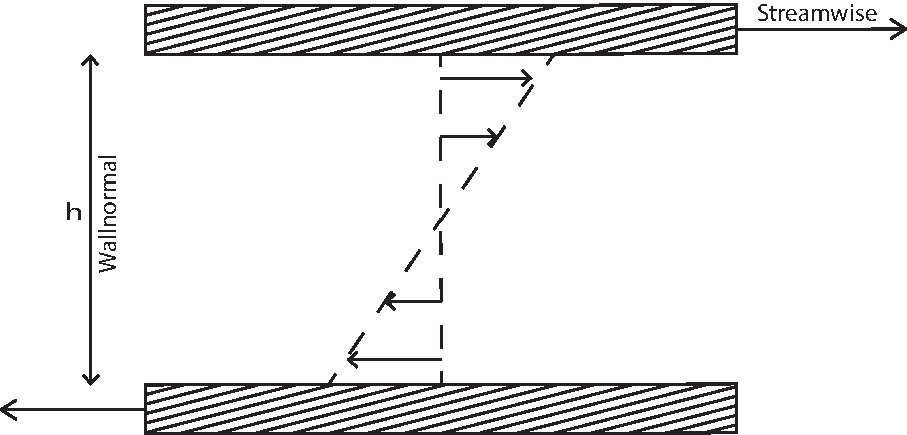
\includegraphics[scale=0.6]{Data/planeCouette}
\end{frame}
\begin{frame}{The System}{Plane Couette}
  The following geometry and assumptions are made
  \begin{enumerate}
    \item {Fluid is constrained between two infinite parallel plates, each with some constant velocity}
    \item {No-slip boundary conditions at the plates}
    \item {Flow is unidirectional: $[u,v,w](x,y,z) = u(y)$}
\item{$\nabla p = 0$}
\item{Gravitational effects are negligible} 
  \end{enumerate}  
\end{frame}

% general installation instructions
\begin{frame}{The System}{Plane Couette}

Under these assumptions, the Navier-Stokes equations reduce to a trivial ODE:
\begin{equation}
\dfrac{\mathrm{d}^2 u}{\mathrm{d}y^2} = 0,
\end{equation}
with boundary conditions $u(0) = 0$, $u(h) = V$ (for example), which gives the bulk flow solution
\begin{equation}
u(y) = u_0 \dfrac{y}{h}.
\end{equation}
\end{frame}

\subsection{Perturbations}
% installation on GNU/Linux
\begin{frame}{The System}{Perturbations}
If we relax the unidirectional requirement on the flow, we can use the Reynolds Decomposition to decompose the new flow field into the sum of the mean flow and a perturbation from it. In this case, we can get $\Vector{u}' = \Vector{u}_{bulk} + \Vector{u}$, where $\Vector{u}$ is a perturbation from the bulk flow. Then we get the following equation for $\Vector{u}$:
\begin{equation}
\dfrac{\del \Vector{u}}{\del t} + y\dfrac{\del \Vector{u}}{\del x} + v\hat{\Vector{x}} + \Vector{u}\cdot\nabla\Vector{u} = \dfrac{1}{\mathrm{Re}}\nabla^2\Vector{u},\hfill \nabla\cdot\Vector{u} = 0
\end{equation} 
\end{frame}

\section{State Space}
\subsection{Hopf's Vision}
\begin{frame}{State Space}{Hopf's Vision}
\begin{itemize}
\item<1-> Fluid flow as trajectories in an infinite dimensional phase space
\item<2-> However, viscosity forces trajectories to lie on some finite-dimensional manifold
\item<3-> Can we map out this manifold? How does it depend on velocity?
\end{itemize}
\end{frame}
\subsection{65,000 dimensions}
\begin{frame}{State Space}{65,000 dimensions}
\begin{itemize}
\item<1-> Divide computational domain into 3D grid
\item<2-> Track components of vector field at each grid point
\item<3-> The state space vector can then be written as $\Vector{v} = (u_{11},v_{11},w_{11},u_{12}....)^T$
\item<4-> The dimension of this space is then given by $3N_xN_yN_z$
\end{itemize}
\end{frame}

\section{Coherent Structures}
\begin{frame}{Coherent Structures}{Equilibria}
\begin{itemize}
\item<1-> Apart from the trivial laminar state, there exist other equilibrium states for $\Vector{u}$. 
\item<2-> These appear to wall off the turbulent regions of the phase space
\item<3-> The following solutions were computed by John Gibson and Predrag Civtanovi\'c at Georgia Tech.
\end{itemize}
\end{frame}
\begin{frame}{Coherent Structures}{Equilibria}
\vbox{\vspace{0.1in}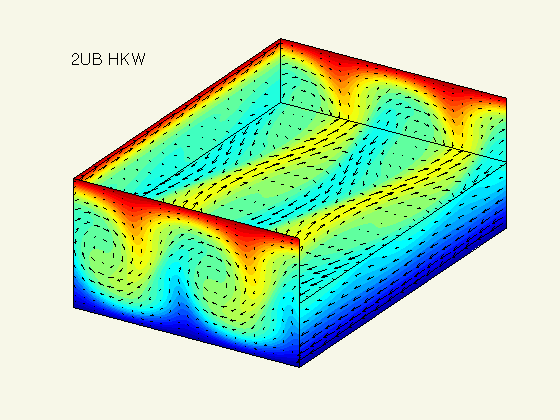
\includegraphics[scale=0.45]{Data/UB}}
\end{frame}
\begin{frame}{Coherent Structures}{Equilibria}
\vbox{\vspace{0.1in}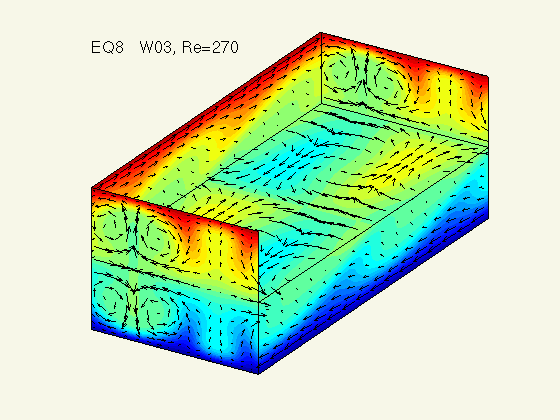
\includegraphics[scale=0.45]{Data/eq8}}
\end{frame}
\subsection{Periodic Orbits}
\begin{frame}{Coherent Structures}{Periodic Orbits}
\begin{itemize}
\item<1-> Limit cycles can also exist
\item<2-> These exist in the middle of the turbulent region of phase space
\item<3-> Do they have some influence on the turbulent dynamics?
\item<4-> Can they help predict tubulent behavior? 
\end{itemize}
\end{frame}
\begin{frame}{Coherent Structures}{State Space}
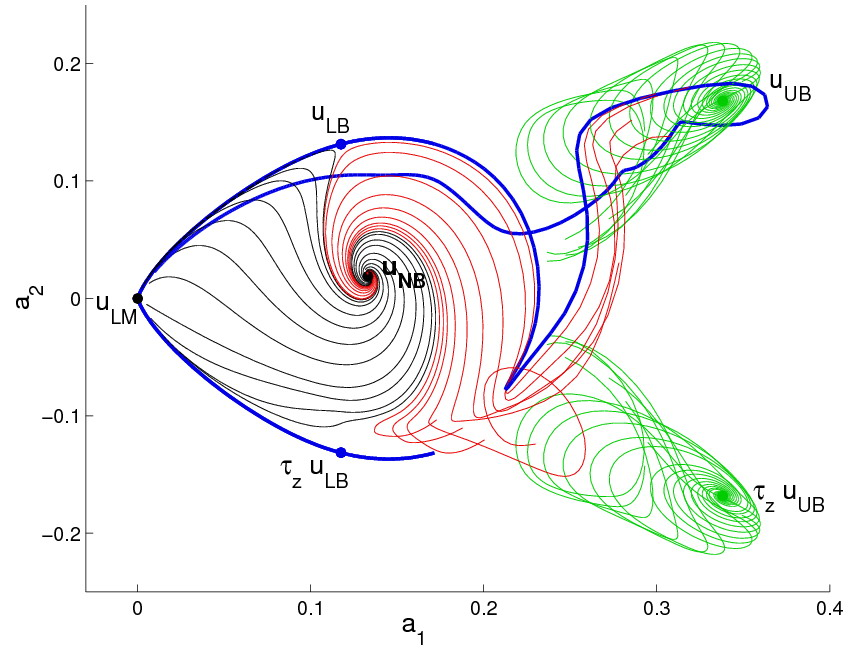
\includegraphics[scale=0.3]{Data/stateSpace}
\end{frame}
\begin{frame}{Coherent Structures}{State Space}
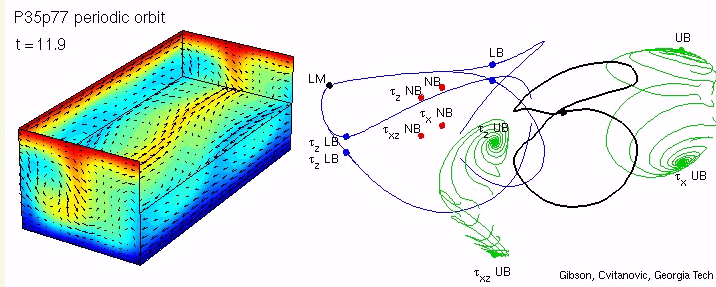
\includegraphics[scale=0.5]{Data/periodicOrbit}
\end{frame}
\section{Symmetry}
\begin{frame}{Symmetry}
The generators of symmetry for $\Vector{u}$ are as follows
\begin{itemize}
\item<1-> $[ u,v,w ](x,y,z) \rightarrow [-u, v, w](-x,y,z)$
\item<2-> $[ u,v,w ](x,y,z) \rightarrow [u, -v, w](x,-y,z)$
\item<3-> $[ u,v,w ](x,y,z) \rightarrow [u, v, -w](x,y,-z)$
\item<4-> $[ u,v,w ](x,y,z) \rightarrow [-u,-v, -w](x,y,z)$
\item<5-> $[ u,v,w ](x,y,z) \rightarrow [-u, v, w](x+l_x,y,z+l_z)$
\end{itemize}
\end{frame}
\begin{frame}{Symmetry}{S Group}
We will limit the explored symmetries to the $S$ group, generated by the following operations:
\begin{itemize}
\item<1-> $s_1[ u,v,w ](x,y,z) =  [u, v, -w](x+0.5L_x,y,-z)$
\item<2-> $s_2[ u,v,w ](x,y,z) =  [-u,-v, w](-x+0.5L_x,-y,z+0.5L_z)$
\item<3-> $s_3[ u,v,w ](x,y,z) =  [-u, -v, -w](-x,-y,-z+0.5L_z)$
\end{itemize}
\end{frame}
%%%%%%%%%%%%%%%%
\section{The Simulation}
\begin{frame}{The Simulation}
\begin{itemize}
\item<1-> I use the software system Channelflow, developed by John Gibson, to simulate the fluid flow and to solve for periodic orbits and equilibria. 
\item<1-> The minimum viable cell is used to speed up computation, with nondimensionalized lengths of $L_x = 1.75\pi$, $L_z = 1.2\pi$ and parallel plates at $y=\pm 1$
\item<2-> Periodic boundary conditions are imposed in the streamwise and spanwise directions, Dirichlet boundary conditions at the plates.
\item<3-> This restricts the size of observable features in the physical flow
\end{itemize}
\end{frame}
\begin{frame}{The Simulation}{The Hunt for the Red October}
\begin{itemize}
\item<1-> How do we hunt through the immense phase space? (> 60,000 dimensions)
\item<2-> Start from a random initial condition
\item<3-> Integrate flow forward in time
\item<4-> Look at recurrence diagrams
\end{itemize}
\end{frame}
\subsection{Recurrence Plots}
\begin{frame}{The Simulation}{Recurrence Plots}
\begin{itemize}
\item<1-> We first need to define a distance function between two flow states
\item<2-> The physically motivated energy norm is used
\end{itemize}
\pause
\begin{equation}
d(\Vector{u},\Vector{v}) = \frac{1}{V}\int_V{\Vector{u}\cdot\Vector{v}}{dV}
\end{equation}
\begin{itemize}
\item<1-> We can now compare the flow at time $t$ to time $t+T$ by calculating $d(\Vector{u}(t),\Vector{u}(t+T))$
\item<2-> Minima of these plots should indicate the presence of a periodic orbit
\end{itemize}
\end{frame}
\subsection{Root Finding}
\begin{frame}{The Simulation}{Root Finding}
\begin{itemize}
\item<1-> Once a promising candidate is found, it can be passed on to the root finder, to solve 
\begin{equation}
\Vector{u} - f^T(\Vector{u}) = 0
\end{equation}
\item<2-> The root finder primarily uses the Newton method, using the generalized minimum residual method to determine the Newton step. 
\item<3-> If the Newton step isn't good enough, a different step $x_H$ is used, which minimizes $||\mathbb{A}x_h - b||^2$.
\item<4-> As opposed to the Newton step $x_N$ which solves $\mathbb{A}x_N = b$ 
\end{itemize}
\end{frame}
\section{The Work}
\subsection{Recurrence Plots}
\begin{frame}{The Work}{Recurrence Plots}
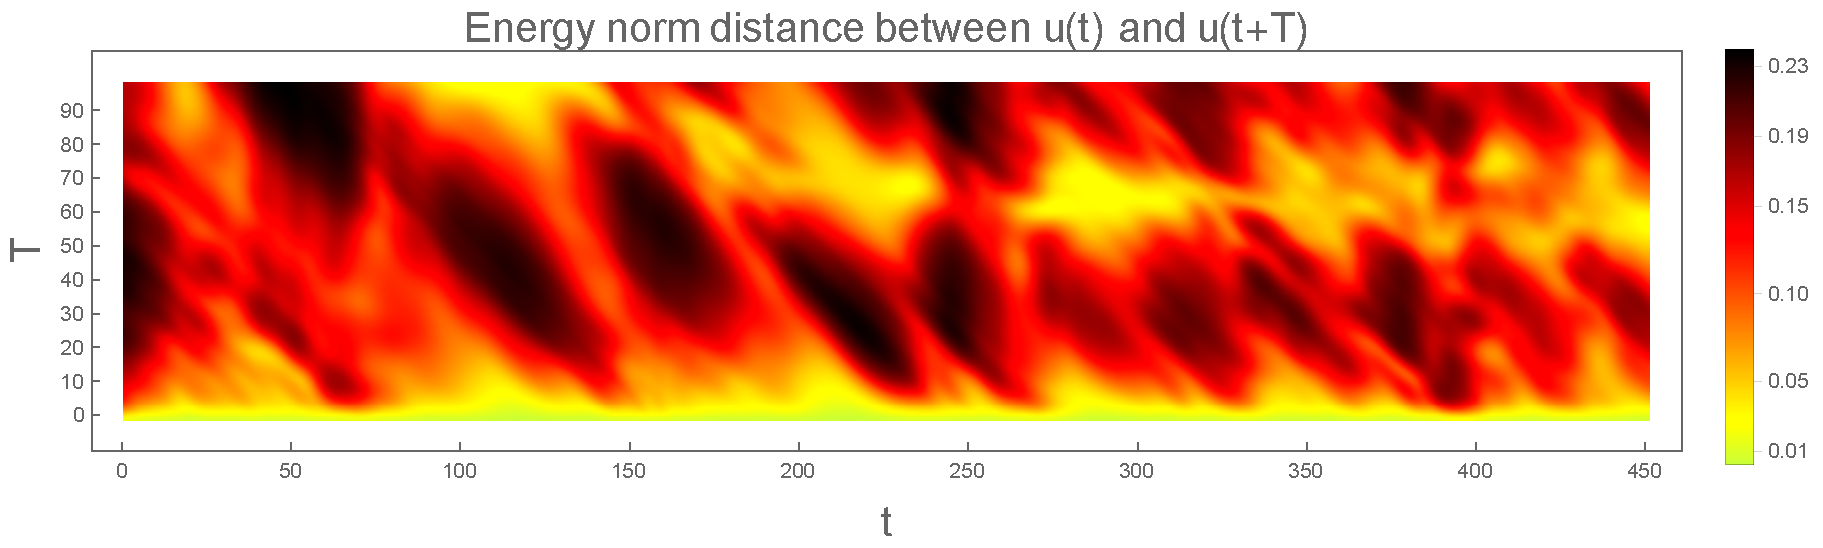
\includegraphics[scale = 0.3]{Data/RecPlot}
\end{frame}
\begin{frame}{The Work}
This orbit has period $T = 85.47$, and has symmetries that are not part of $S$. 
\vbox{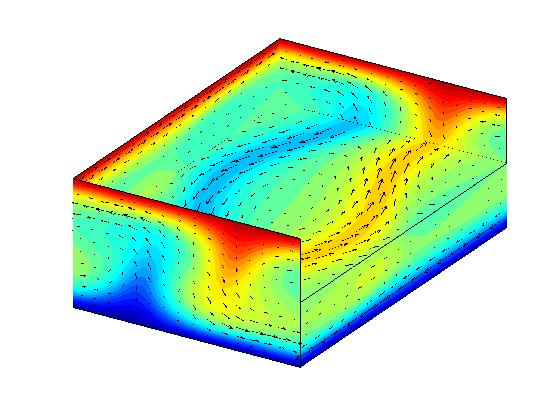
\includegraphics[scale=0.45]{Data/p85-47}}
\end{frame}
\begin{frame}
\vbox{\vspace{20mm}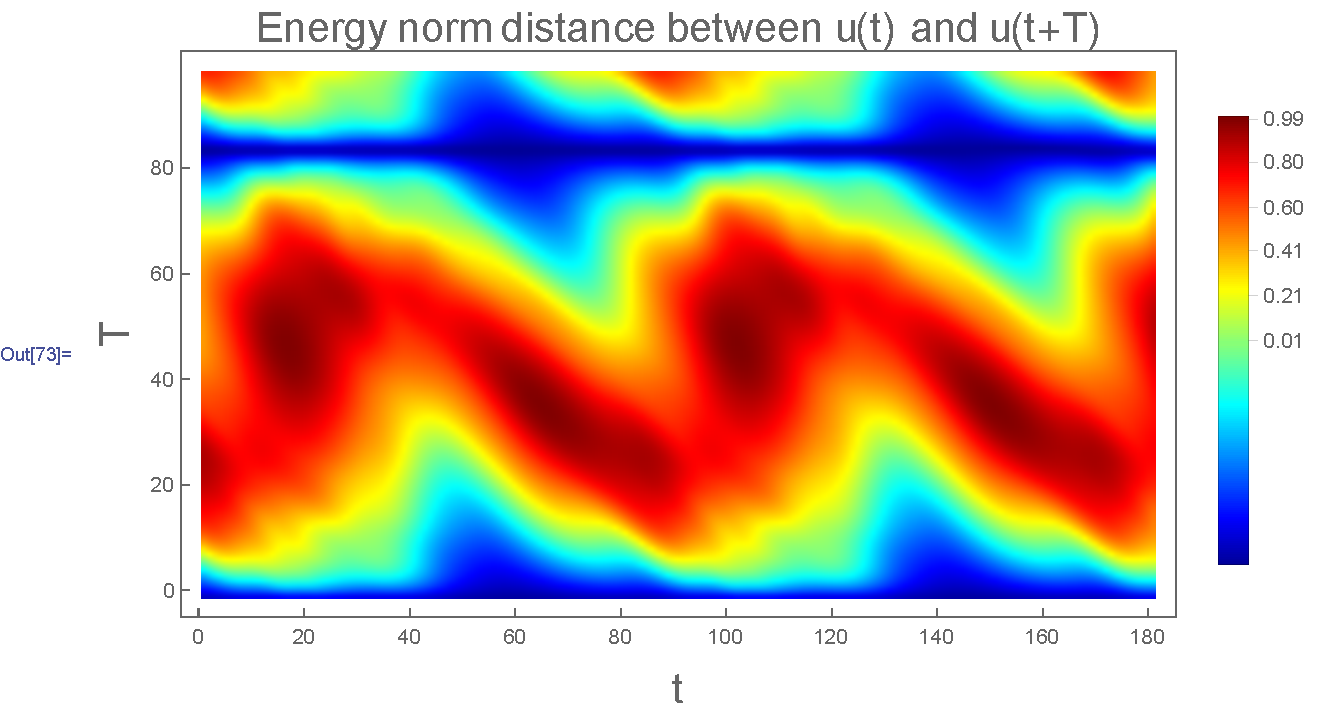
\includegraphics[scale=0.40]{Data/p85p47Rec}}
\end{frame}
\begin{frame}
\includegraphics[scale=0.4]{Data/randomfield}
\end{frame}
\begin{frame}{Future Work}
\begin{itemize}
\item<1-> Locate more periodic orbits in the symmetric subspace
\item<2-> Remove symmetry constraints and attempt to locate asymmetric orbits
\end{itemize}
\end{frame}
\begin{frame}
\begin{figure}
\begin{tabular}{cc}
\includegraphics[scale=0.2]{Data/randomfield} & 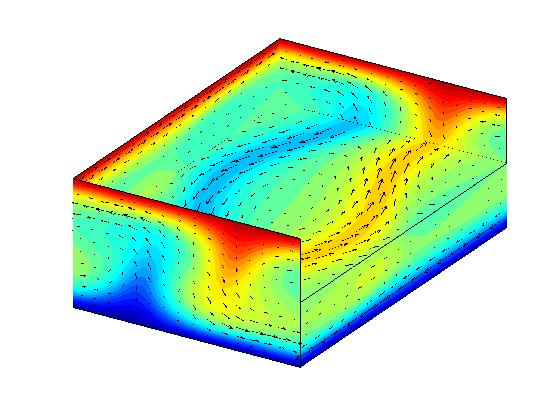
\includegraphics[scale=0.2]{Data/p85-47}\\
A random field & A highly symmetric field
\end{tabular}
\end{figure}
\end{frame}
{\aauwavesbg%
\begin{frame}[plain,noframenumbering]%
  \finalpage{I'd like to thank the following people for making the progress so far possible:  
\begin{itemize}
\item<1-> John Gibson at UNH and Predrag Civitanovi\'c at Georgia Tech for making the subject approachable
\item<2-> Daniel Borrerro for putting up with my lack of progress
\end{itemize}}
\end{frame}}
%%%%%%%%%%%%%%%%

\end{document}
